%%%%%%%%%%%% MAIN PACKAGES %%%%%%%%%%%%
\documentclass{template}
\usepackage{graphicx,parskip,appendix,float}
\graphicspath{ .{images/} }
\usepackage{fontawesome5}
\usepackage[ruled]{algorithm2e}
\usepackage{url,amsmath,amssymb,fancybox,listings,pdfpages,caption,multicol,datetime,rotating, booktabs}
\usepackage{csquotes}
\usepackage{nameref}
\usepackage{minted}
\usepackage{xcolor}
\usepackage{nomencl}
\makenomenclature
%\usepackage[usenames,dvipsnames]{color} % Don't use it, as it clashes with csquote
% NOTE: When pagebackref=true an error will appear at the end of compiling. press `q' to ignore
% NOTE: Referencing Algorithms does not work if this usepackage is before the hyperref include.!!
% NOTE: More packages may need to be added to provide additional functionality
%%%%%%%%%%%%%%%%%%%%%%%%%%%%%%%%%%%%%%%%%%%%%%%%


%%%%%%%%%%%% LINE NUMBERS %%%%%%%%%%%%
% NOTE: If you want to add line numbers to your document and make it easier for markers to provide you feedback, uncomment the following two lines
%\usepackage{lineno}
%\linenumbers
%%%%%%%%%%%%%%%%%%%%%%%%%%%%%%%%%%%%%%%%%%%%%%%%


%%%%%%%%%%%% REFERENCING STYLES %%%%%%%%%%%% 
% NOTE: Comment/Uncomment based on preference or requirement

\usepackage[style=authoryear,giveninits,backend=biber]{biblatex} % Harvard, RGU prefers this
\renewcommand*{\nameyeardelim}{\addcomma\space}

% \usepackage{biblatex} % Vancouver, most people prefer this as it is simpler to follow!

% NOTE: The command below imports your references from thesis.bib
\addbibresource{thesis.bib}
%%%%%%%%%%%%%%%%%%%%%%%%%%%%%%%%%%%%%%%%%%%%%%%%


%%%%%%%%%%%% TRACK CHANGES AND ANNOTATIONS %%%%%%%%%%%
% NOTE: If you want to add notes, highlight or have your supervisor track changes, we recommend using these packages
% TodoNotes: https://tug.ctan.org/macros/latex/contrib/todonotes/todonotes.pdf
% Soul: https://cs.brown.edu/about/system/managed/latex/doc/soul.pdf

%\usepackage{todonotes}
%\usepackage{soul}
%%%%%%%%%%%%%%%%%%%%%%%%%%%%%%%%%%%%%%%%%%%%%%%%


%%%%%%%%%% HYPERREF %%%%%%%%%%%%
% NOTE: This package highlights links to your sections/chapters in the compiled pdf, which is always good to have. For this package to work properly, it has to be the last one to be declared
\usepackage[pagebackref=false,pdffitwindow=true]{hyperref} 
%%%%%%%%%%%%%%%%%%%%%%%%%%%%%%%%%%%%%%%%%%%%%%%%


%%%%%%%%%% DOCUMENT CONFIGURATION SETTINGS (ignore unless you really need to change something!) %%%%%%%%%%%%
\hypersetup{
    pdftitle    = {PropertyIQ: Explainable Decision-Support System (DSS) for UK Residential Property Investment},
    pdfauthor   = {Milen Kirilov},
    pdfsubject  = {Machine Learning},
    pdfkeywords = {Machine Learning, DSS, XAI, Property, SHAP, XGBoost},
    colorlinks  = true, anchorcolor = blue, filecolor = blue, urlcolor = blue,
    linkcolor   = blue, % NOTE: change (blue) to (colIdentifier) to have links within the document in Black
    citecolor   = blue, % NOTE: change (blue) to (colIdentifier) to have citation links within the document in Black
}

\definecolor{colBackGrnd}{rgb}{1,1,0.8}
\definecolor{colKeys}{rgb}{0,0,1}
\definecolor{colIdentifier}{rgb}{0,0,0}
\definecolor{colComments}{rgb}{0,.5,0}
\definecolor{colString}{rgb}{0,0,1}
\definecolor{colWhite}{rgb}{1,1,1}

\newcommand{\MyHookSign}{\hbox{\ensuremath\hookleftarrow}}

\newtheorem{Theorem}{Theorem}
\newtheorem{Proposition}[Theorem]{Proposition}
\newtheorem{Lemma}[Theorem]{Lemma}
\newtheorem{Proof}[Theorem]{Proof}
\newtheorem{Remark}[Theorem]{Remark}
\newtheorem{Claim}[Theorem]{Claim}
\newtheorem{Example}[Theorem]{Example}
\newtheorem{Definition}[Theorem]{Definition}

% NOTE: Setup for including program listings
\lstset{%
    float=H,
    basicstyle=\ttfamily\footnotesize,
    identifierstyle=\color{colIdentifier},
    keywordstyle=\color{colIdentifier}, %
    stringstyle=\color{colIdentifier},
    commentstyle=\color{colIdentifier}, %
    columns=flexible,
    tabsize=2,
    frame=single,
    extendedchars=true, %
    showspaces=false,
    showstringspaces=false,
    numbers=left, %
    numberstyle=\footnotesize,
    breaklines=true,
    prebreak={\space\MyHookSign},
    language=Java,
    backgroundcolor=\color{colBackGrnd},
    breakautoindent=true, %
    captionpos=b%
} %\hypersetup{colorlinks=true, citecolor=\color{colIdentifier}}

\sloppy % NOTE: To ensure the Right Hand Margin is used (Especially for long URLS)
% NOTE: END of the document configuration settings
%%%%%%%%%%%%%%%%%%%%%%%%%%%%%%%%%%%%%%%%%%%%%%%%


%%%%%%%%%% YOUR DOCUMENT %%%%%%%%%%%%
\begin{document}
\DeclareGraphicsExtensions{.jpg,.png,.gif,.pdf} % When inserting Figures, if the extension of the graphic file is not provided LaTeX will automatically search for the extensions declared above, in the order declared

% Replace accordingly
\title{\huge{PropertyIQ: Explainable Decision-Support System (DSS) For UK Residential Property Investment}}
\author{Milen Kirilov}
\degreetitle{BSc Hons Computing (Application Software Development)}
\rpttype{Degree}
\principaladviser{Ross McLean}

\beforeabstract
\prefacesection{Abstract}

This project examines the advantages and development of Machine Learning (ML) models designed to \textbf{explain the factors influencing property values in natural human language}.

The project is divided into two primary components: implementing eXtreme Gradient Boosting (XGBoost) to predict property values based on specific features (e.g. square metres, number of bedrooms) and utilising SHapley Additive exPlanations (SHAP) to articulate, in human language, the rationale behind the model's evaluation. 

The literature review underscores several benefits of eXplainable Artificial Intelligence (XAI) within the property market sector, highlighting the significance for end users receiving detailed, human-readable explanations of the factors affecting the model's judgement, as opposed to a mere score system, where the model's reasoning remains opaque. 

The chosen model for the task, XGBoost, is a gradient-boosting decision-making machine learning model that parallels the human evaluation of property values in the market by considering various attributes and generating an overall estimate based on the data provided during model training. Following the predictions of XGBoost, SHAP identifies the features that have increased or decreased the prediction values and quantifies their impact, ultimately generating explanatory text based on the influence of different features of the dataset.

\prefacesection{Acknowledgments}
I express my sincere gratitude to my project supervisor, Ross McLean, for his guidance throughout this project and for his assistance in resolving the various challenges I encountered along the way. His professionalism and dedication have been truly exceptional and I consider myself fortunate to have worked under his supervision.

I extend my thanks to the entire School of Computing, Engineering and Technology at the Robert Gordon University for the knowledge, support, and formative experiences that have shaped me into a better version of myself. I expressly acknowledge professor John N. Brown, whose teaching broadened my perspective and encouraged me to think critically and beyond conventional boundaries. 

I would like to dedicate this work to my mother and father, whose sacrifices and unwavering support have made it possible for me to reach this point; and to my brother, whose presence has been a constant source of strength. I am also very thankful to my aunt, who cared for me as if I were her own child.

Finally, my heartfelt thanks go to my girlfriend, Ivana, who stood with me throughout this glorious journey. Not for a single moment did she stop believing in me. Even in the moments when I was at my lowest, mentally and physically, and ready to give up, she refused to let me do so. Her encouragement and unwavering faith carried me to the finish line, and for that I will always be grateful.

\afterpreface \afterabstract
%\listofalgorithms % NOTE: Will generate a list of Algorithms in the Table of Contents Section
%\lstlistoflistings % NOTE: Will generate a list of Program Listings in the Table of Contents Section

% NOTE: Include the relative reference for each chapter to be included
% dividing the thesis file structure into a number of directories aids development
% format: directoryName/filename (the .tex extension is not required for the filename)
\chapter{Introduction}
\pagenumbering{arabic} \setcounter{page}{1}

This project presents PropertyIQ: a web-based application designed to offer unambiguous insights into properties available on the market through the use of ML models, and it has been uploaded and can be found on GitHub \parencite{Kirilov2026}. This project introduces an \textbf{innovative methodology for comprehending property values} by leveraging known attributes that characterise and define a property while incorporating external factors such as the quality of the location.              

PropertyIQ is constructed using two complementary machine learning models: the first model predicts the value of a property based on the property features and facilitates a comparison with existing properties on the market, while the second model analyses the resulting valuation and generates human-readable explanations of the predicted price. 

Both models were trained on a dataset generated by scraping Zoopla \parencite{Data2024}, which contains real-world values from existing properties with detailed features.

This project aligns with Goal 9 of the Sustainable Development Goals of the United Nations: \textit{build resilient infrastructure, promote inclusive and sustainable industrialisation, and foster innovation} \parencite{UnitedNations2011}. PropertyIQ advances the \textbf{inclusive industrialisation} pillar by democratising access to property valuation, enabling users to obtain a credible estimate of a property's market value regardless of prior appraisal expertise and thereby reducing the knowledge required that has historically disadvantaged first-time buyers, small landlords, and less affluent market participants. It further contributes to the \textbf{innovation} pillar by adopting a system that, although well-established in the academic machine-learning literature, remains insufficiently exploited in the property market: model prediction explainability. Rather than returning a single opaque estimate, the system decomposes the prediction into the contribution of individual property features, allowing users to interrogate the given valuation that has been produced; as discussed in Section~\ref{se:GeneralBenfits} \nameref{se:GeneralBenfits}. This transparency is of substantial practical benefit to non-expert users, who require not just a figure but a justification on which to base a significant financial decision.


\section{Motivation and Objectives}

This project seeks to address the existing gap between the application of Artificial Intelligence (AI) systems that solely assess a property's value and the necessity to comprehend the rationale behind such valuations. PropertyIQ aims to rectify this deficiency by integrating predictive modelling with XAI techniques, enabling users to engage with both the valuation process and its underlying justification. 

The following objectives for this project have been identified.

\begin{enumerate}

  \item \textbf{Achieve accurate property valuations} using ML, by training a regression model on real-world UK property data to produce reliable value estimates based on a defined set of property features.
  
  \item \textbf{Ensure transparent and comprehensible explanations} by employing a machine learning technique to decompose each valuation into the individual contributions of each feature, which are then translated into plain English that is accessible to non-technical users.
  
  \item \textbf{Provide a comprehensive understanding of valuations} within the market; it is essential to present each predicted value in conjunction with comparable properties from the dataset. This will also allow users to assess the estimate by comparing it with similar listings in the same geographical area rather than evaluating it in isolation.
  
  \item \textbf{Facilitate informed decision-making} in the property market by elucidating the factors underlying property valuations and encourage individuals to critically evaluate property estimates rather than accepting them uncritically, thus mitigating the risk of overconfidence, which may result in excessive expenditure over time.
  
  \item \textbf{Develop an accessible web-based interface} that is suitable for prospective buyers, small-scale investors, and property researchers without requiring technical expertise in machine learning or property investment.
  
  \item \textbf{Establish a scalable and maintainable framework} in which the underlying dataset, model, and explanation pipeline can be extended on new data. This approach will facilitate future development beyond the scope of this project.
  
\end{enumerate}



\chapter{Background Research}\label{ch:Background}

Residential property appraisal has historically been grounded in a limited set of established methodologies, within which the determination of value and its accompanying justification were produced in a single act with a single result. The artefact that generated the valuation (whether an appraiser's written commentary, a grid of adjustments applied to comparable transactions, or a regression coefficient) simultaneously constituted the evidentiary basis for that valuation \parencite{Pagourtzi2003}.

This relationship between method and explanation becomes especially important when we consider what happens if traditional human appraisers are replaced by predictive models that generate a single output value, creating a loss of trust and reliability in the prediction value \parencite{Pagourtzi2003}.

In the sales comparison approach, for example, the value of a property is estimated by looking at recent sales of similar properties, then manually adjusted for differences that differ between the properties (e.g. size, condition, and location) \parencite{Pagourtzi2003}

What makes this approach transparent is the appraiser's written report. Every comparable property chosen is explained, and every adjustment is justified in plain language, meaning anyone reading the report can follow the logic from start to finish. However, these judgments are ultimately subjective and cannot be fully standardised.

As a result, two appraisers looking at the same property may reach different conclusions, and the method has faced ongoing academic criticism for lacking objectivity and consistency \parencite{Pagourtzi2003}.

To address the issue, the \textbf{hedonic pricing model} emerged as a statistical formalisation of the comparative approach and represents the earliest systematic attempt to produce a per-feature explanation of residential property prices. Building on the theoretical foundation of \textcite{Rosen1974}, hedonic models decompose a property into its structural, locational, and environmental characteristics and use multiple linear regressions to estimate the marginal contribution of each attribute to the overall price. Due to these factors, hedonic models became dominant in mass appraisals because of their explanatory transparency: each regression coefficient carries a direct economic interpretation, and the contribution of every feature to the predicted value can be stated numerically and in human-readable terms \parencite{Wing2003}.

In this sense, hedonic regression is the direct conceptual ancestor of the feature-attribution approach, which was later pursued in XAI \parencite{Iban2022}. 

However, hedonic models rest on the assumption that the relationship between property attributes and price is linear and additive, an assumption that has been repeatedly shown to be violated in real housing markets, where interactions between location, amenities, and structural characteristics are inherently non-linear \parencite{Wing2003}.

The methods that were explainable by construction could not capture the true complexity of the market, while the methods capable of capturing that complexity would, by their nature, sacrifice the interpretability on which traditional valuation has always relied \parencite{Lorenz2023}.


\section{General Benefits of Property Valuation Explanation}
\label{se:GeneralBenfits}

One of the primary advantages of explaining a property's value is \textbf{fostering user trust when using ML models}.

\textcite{Ribeiro2016} demonstrates that users show a significantly greater likelihood to accept and act upon a model's output when the prediction is accompanied by a human-interpretable rationale rather than presented as a raw score; and this consideration carries particular weight in the real estate domain, where valuations inform long-term investments and purchase decisions. The costs of misplaced confidence are correspondingly high. For example, when the reasoning is made explicit, such as how a larger floor area or good public transport proximity increases the value of the property, while poor property condition decreases it, users can assess whether the valuation makes sense based on their knowledge about the market. Thus, \textbf{users are not simply forced to accept a score to base their judgement on, but can evaluate the process and the factors that influenced the decision of the model}.

Furthermore, articulating property valuation has educational benefits. As users are exposed to the attributes that shape a given estimate and the magnitudes of their respective contributions, they progressively acquire a more sophisticated understanding of the market in which they consider participating. This is of particular consequence for first-time home-buyers, who typically lack the experiential grounding required to assess whether a given property is fairly priced and report corresponding uncertainty in their decision-making \parencite{Reid2013}. 

In this context, explanation serves not only to \textbf{legitimise individual valuations} but also to \textbf{cultivate the user's evaluative competence} over time. By making the reasoning behind each estimate visible, an explainability platform moves away from presenting itself as an infallible authority on property values. Instead, it offers an informed prediction; one the user can question, weigh against their own knowledge, and use as a starting point for deeper understanding.

In this way, explainability converts what would otherwise be a silent output, a single figure, delivered without elaboration, into an instructive resource that accompanies the user throughout the decision.


\section{Use of Property Valuation Explanation}

The precise evaluation of the values of residential properties is crucial for a wide array of financial decisions made by both institutional entities and individual investors. \textcite{Gray2021}  highlight that \textbf{a substantial portion of global wealth is vested in real estate}, with significant financing contingent upon the accuracy of property valuations.

This positions properties as a fundamental component of the financial system.
In the lending sector, property valuations are used by banks and building societies to ascertain the loan-to-value ratio, thereby influencing the associated risk and interest rate of mortgages \parencite{Gan2008}. For individual investors, the perceived value of a property directly affects the cost and availability of the necessary financing for acquisition, rendering valuation reasoning a matter of immediate practical significance rather than a professional concern.
For small-scale and individual investors, property values guide decisions related to acquisition, disposal, and long-term wealth accumulation. 

\textcite{Johnson2024} assert that valuation outputs are essential not only for pricing individual assets but also for securing lending, indicating that the quality of valuation directly impacts an investor's market entry and sustainability. In this context, demystifying the rationale behind the value of a property, rather than simply reporting a figure, allows users to evaluate the underlying assumptions regarding rental yield, growth potential, and location risk \parencite{Gabrielli2021}. 

This examination is particularly vital for non-professional investors, who typically lack access to qualified surveyors and proprietary data sources available to institutional participants, and must therefore rely on publicly accessible information to assess opportunities.
As a result, an explainable valuation holds practical significance for individual households and small-scale investors, who depend on interpretable evidence to make financially significant decisions, often representing their largest financial commitments \parencite{Rinaudo2025}.


\section{Machine Learning in Property Valuation Explanation
\label{se:MLBackground}}

The uptake of ML in property valuation has grown substantially alongside the availability of larger and geo-referenced housing datasets \parencite{Kang2021}. Large \textbf{datasets enable ML algorithms to capture non-linear relationships} that are typically difficult to estimate using traditional hedonic price models \parencite{Ho2020}.

The results from the literature show that ensemble models, specifically Random Forest (RF) and Gradient Boosting, outperform Linear Regression and Support Vector Machines in standard error metrics, including Mean Squared Error (MSE), Root Mean Squared Error (RMSE), and Mean Absolute Percentage Error (MAPE). Tree-based algorithms also exceeded the predictive accuracy of other models in the South Korean housing market  \parencite{Hong2020}. 

\textcite{Rico-Juan2021} found similar results when they used ML models to outperform spatial hedonic models in predicting asking prices in Alicante, Spain. However, these gains in predictive performance are typically offset by a loss of interpretability; a limitation widely termed the ``black-box'' problem. The concern is severe in settings where transparency is a prerequisite rather than a convenience, including property taxation, mortgage lending, and mass appraisal. 

In response, a growing body of work has turned to XAI techniques, SHAP and Permutation Feature Importance (PFI) foremost among them, to quantify how individual property attributes contribute to predicted values. A study carried out by \textcite{Kim2025} demonstrates that SHAP enables both global and local explanations of non-linear effects, revealing threshold behaviours that hedonic regressions cannot capture.

Furthermore, the opacity of complex predictive models has driven growing interest in XAI, broadly defined as the set of processes that allow stakeholders to understand how an AI system arrives at its predictions and decisions. Within the information systems literature, XAI has been positioned as a critical enabler of AI-driven Decision Support Systems (DSS) \parencite{Giudice2019}, where the output of the model alone is insufficient; the reasoning behind it must also be interpretable for the system to support informed decision-making \parencite{Meske2022}. 

This is particularly pertinent in residential property valuation, where the transition from transparent hedonic regression models to high-capacity ensemble methods introduced a fundamental trade-off between predictive accuracy and interpretability \parencite{Gunes2024}.

\section{Summary}

This review of the literature aims to summarise current research on factors influencing house prices. This field of study has recently expanded to utilise ML techniques to predict and explain housing prices. 

Hedonic regression, formulated by \textcite{Rosen1974}, has been the foundation of modern real estate appraisal, valuing properties based on implicit prices of structural, location, and neighbourhood characteristics, owing to its interpretability advantage \parencite{Wing2003}. 

However, it has been shown that these assumptions of parametric models are no longer valid due to dynamic housing markets \parencite{An2025} and human bias, as manual appraisal lacks consistency between valuers \parencite{Aluko2007}. 

However, it has been shown that the linearity and additivity assumptions underpinning parametric models are inadequate for capturing the dynamic and nonlinear behaviour of modern housing markets \parencite{An2025}, whilst manual appraisal is itself constrained by human bias and a well-documented lack of consistency between appraisers.

The solution has been for academics to apply ML algorithms to property data and find that ensemble methods such as FR and Gradient Boosting outperform regression on the predictive accuracy benchmark \parencite{eh2018};. 

The explainability of property value has large real-world applications, from enabling mortgage loans to assisting in taxation, investment, and city planning \parencite{Iban2022}. Therefore, accuracy is not enough, and regulators and end-users demand interpretable models \parencite{Lorenz2023}. 

This has been an issue of ML models labelled as the ``black-box'' problem \parencite{Adadi2018}, and efforts have been made to utilise XAI techniques, including SHAP and Local Interpretable Model-Agnostic Explanations (LIME), in the housing domain \parencite{Lundberg2017} \parencite{Ribeiro2016}.

Recent studies by \textcite{Rico-Juan2021} and \textcite{Iban2022}, have shown that SHAP can recover the directional and quantitative effects of hedonic variables from a RF or XGBoost model, offering a credible compromise between accuracy and explainability. Given this evidence, it is reasonable to assert that an ML-based valuation tool should be complemented by a model-agnostic explanation layer, providing users with a predicted price and a justification grounded in the specific characteristics of the property. 

However, existing research has predominantly focused on data from markets such as Hong Kong \parencite{Ho2020}, Korea \parencite{Kim2025}, Spain \parencite{Rico-Juan2021} and Turkey \parencite{Iban2022}, and has concentrated on producing academic analyses rather than end-user-facing tools. Relatively little research has explored how these explanations should be presented to non-expert buyers and sellers in practical applications \parencite{Bauer2023}. 

Thus, this literature review offers valuable insight into both the \textbf{technical maturity of explainable property valuation and the relative lack of user-orientated implementations}, which together justify the direction taken in this project.

\chapter{Design and Methodologies}\label{ch:Design}

The PropertyIQ design is based on the belief that transparency and explainability are essential for developing reliable decision-support systems. 

The web-based application directly addresses the identified limitations of existing property platform tools, which often present scores and rankings without revealing the underlying reasoning. 

\textcite{Ribeiro2016} highlighted the importance of user-centric transparency, arguing that \textbf{decision-support tools are effective only when users can comprehend and trust their outputs}, thus, the PropertyIQ web application was designed to generate predictions and explain them. 

Furthermore, following the approach advocated by \textcite{Lundberg2017}, PropertyIQ combines predictive modelling with interpretability. XGBoost \parencite{Chen2016} is used to generate property valuations, whereas SHAP \parencite{Lundberg2017} values decompose each prediction, attributing a quantified contribution to every input feature and presenting it in a human-understandable language.

The modular system architecture is structured into two distinct layers: a JavaScript React \parencite{Meta2026} frontend, which is responsible for filtering and visualisation, and a Python Uvicorn \parencite{Trylesinski2026} backend, which handles data transformation and serves the processed property data through the Representational State Transfer (REST) API endpoints \parencite{Powell2025}.

Although both layers are deployed from the same Uvicorn process, the clear separation between presentation logic and data processing logic enhances the readability and maintainability of the codebase.

PropertyIQ implements a strategy of progressive disclosure of complexity, ensuring accessibility to non-expert investors by providing immediate and actionable insights by highlighting risk indicators, such as short remaining leaseholds, high EPC ratings, and council tax bands. This approach transforms raw data into an interpretable system, enabling users to \textbf{understand the rationale behind the valuation of properties derived from machine learning}.

On a side note, the development of PropertyIQ reflects the three foundations of professionalism articulated by the British Computer Society \parencite{BSC2022}. \textbf{Socially}, the system reduces the informational inequality between professional intermediaries and ordinary market participants by offering transparent, explainable valuations to non-expert users, while being framed as a decision-support tool rather than a substitute for professional judgement. \textbf{Legally}, it complies with the UK GDPR \parencite{GDPR2016} and the Data Protection Act 2018 \parencite{DPA2018}: only legally obtained non-personal property data are used, and the explainability layer aligns with the interest of the data-subject in meaningful information on automated decision-making. \textbf{Ethically}, the project follows the BCS Code of Conduct: the model has been evaluated for predictive performance and potential socio-geographic bias, its limitations are communicated openly rather than concealed behind a single confident figure, and explainability exists so that users may exercise informed judgement rather than defer uncritically to the model.


\section{Implementation Strategies}

The implementation of PropertyIQ requires an iterative development process that involves the integration of machine learning pipelines into the web application.

The initial phase focused on data exploration and preparation. The dataset, a Comma Separated Value (CSV) file, obtained by scraping Zoopla and containing 1,000 UK residential property listings with 43 attributes, was imported using the Pandas \parencite{Pandas2026} library. Feature engineering was used to extract investment-relevant signals from raw attributes, such as price, size, and EPC rating.

The second phase focused on model development, where XGBoost was chosen due to its interpretability and ease to implement; while more advanced and complex algorithms such as neural networks may have yielded a more accurate prediction, which adds a level of complexity to this project without increasing the explanatory features \parencite{Sharma2024}.

Thereafter, the trained XGBoost model was integrated  with SHAP to produce natural language explanations of how individual property features affected valuation of the price for the property; and this ML pipeline was developed before being integrated into the backend.

Following the validation of the model, the third phase involved the integration of the ML pipeline into a Python backend, which was deployed using Uvicorn to provide RESTful API endpoints accessible via the React frontend, facilitated by Vite \parencite{VoidZeroInc2026}.


\section{Development Tools}

The following tools have been used throughout this project development and in order to create the two ML models (XGBoost and SHAP) and  develop the React web app of PropertyIQ.

\begin{itemize}
    \item PyCharm \parencite{JetBrains2026} served as the primary Integrated Development Environment (IDE), with extensions configured to support both Python and JavaScript React workflows.
    
    \item Jupyter Notebook \parencite{JupyterTeam2015} was adopted as the principal environment for model development, exploratory analysis, and validation prior to backend integration, due to its interactive execution model and native support for inline visualisation.
    
    \item XGBoost was selected for its well-documented performance on structured tabular data and its natural compatibility with SHAP, the explainability framework employed to derive feature-level contribution scores for individual property predictions.
    
    \item Uvicorn, was chosen for the backend implementation due to its minimal resource footprint and strong interoperability with the broader data science ecosystem.
    
    \item Pandas and Numpy were used for the ingestion and preprocessing of CSV dataset. Although there are more performant alternatives such as Polars \parencite{JodieBurchell2024}, the former libraries were preferred for their widespread adoption within the academic data science and machine learning community, thus improving the accessibility and reproducibility of the development process.
    
    \item React, which was scaffolded via Vite, was selected for its component-based architecture, which aligns with the modular design philosophy of the proposed system. Vite's hot-module replacement capability further accelerated the frontend development cycle.
    
    \item Tailwind CSS \parencite{TailwindLabs2021} was employed for utility-first styling, facilitating rapid interface development without requiring context-switching to separate stylesheet definitions.
    
    \item Recharts \parencite{recharts2026} was used for its Scalable Vector Graphics (SVG) based rendering engine and native React integration, allowing the visualisation of investment indicators and risk distributions throughout the data set.
    
\end{itemize}




\chapter{Implementation}
\label{ch:Implementation}

The implementation of PropertyIQ was based on the design decisions outlined in Section \ref{ch:Design} \nameref{ch:Design}, providing a comprehensive architecture and rationale for selecting XGBoost and SHAP, and integrating the models into the web application.

PropertyIQ is a compact system that comprises a data preparation pipeline, a valuation model, an explanation layer, a Python backend and a React frontend. The significance of this configuration lies in its dual focus: generate a valuation and ensure that this valuation is accessible and comprehensible to the user via the web application. 

The following subsections delineate the logical sequence of the system's construction. Commencing with the development environment and data preparation, progressing through feature engineering and model construction, and culminating in the integration of the back-end and front-end components.

\section{Project Structure and Development Environment}

The implementation of PropertyIQ was structured into three primary layers: a notebook-based machine-learning workspace, a Python backend, and a React frontend. This architecture was adopted at an early stage to facilitate project management and mitigate the risk of merging exploratory modelling and deployment-orientated tasks. 

Initially, the machine learning pipeline was developed within Jupyter Notebook, allowing inspection, cleaning, transformation, and use of the data set to train the regression model, which, consequentially, was used by the explanatory model to articulate the prediction. Once this component achieved sufficient stability, the trained artefacts (in the form of \texttt{.pkl} files \parencite{Oderinwale2025}) were transferred to the backend, allowing their use by the web application.

The development of the model involved iterative experimentation with data preprocessing steps, feature selection, and model configuration. By maintaining the training process within a notebook and the deployment logic in separate Python files, the model was refined without demanding the continual restructuring of large sections of the codebase upon changes.

The frontend was developed using React in combination with Vite, Tailwind CSS, React Router, and Recharts. The backend was implemented using FastAPI \parencite{FastAPI2025} and deployed via Uvicorn. Throughout both the backend and notebook phases, Pandas was employed to process, manage, and manipulate the data.


\section{Dataset and Data Preprocessing}

The initial phase of implementation focused on \textbf{transforming the data inside to be suitable for supervised machine learning}, as the dataset was sourced from scraped Zoopla listings and contained 1,000 rows and 43 columns in its raw form.

Although the data provided a valuable real-world basis for the project, they also introduced typcical challenges associated with data sliced on the web \parencite{Foerderer2023}. A significant number of fields were irrelevant, some were only partially populated, and several values that were inherently numerical were extracted as formatted strings.

The analysis started by importing the CSV dataset file into Pandas and performing an initial examination. This initial assessment promptly indicated that not all available fields would be advantageous for modelling purposes.

Certain columns, such as web URLs, image links, and map references, lacked direct relevance for price prediction \parencite{Kotsiantis2006}. Furthermore, some columns, including \texttt{virtual\_tours}, \texttt{deposits} and \texttt{letting\_arrangements}, were nearly empty of data; thus a more selective data filtering approach was adopted, focusing on fields that could be consistently cleaned and were likely to contribute meaningfully to the ML model valuation task.

A significant component of this phase involved the transformation of string-represented values into numerical counterparts. For example, the variable \texttt{price} was initially presented as a formatted string containing currency symbols and commas, while \texttt{service\_charge} was similarly formatted as an annual, monthly, or weekly amount, and \texttt{property\_size} included unit text rather than a simple number. 

These elements were processed using regular expression-based stripping before conversion into numerical values. In addition, fields such as the number of bedrooms, bathrooms, receptions, and leasehold-related attributes were converted to numerical form where feasible.

Furthermore, certain features, such as \texttt{property\_type}, were standardised to a lowercase value for subsequent encoding (e.g. ``new-homes'' are represented by \texttt{0} and ``for-sale'' by \texttt{1}). Although these procedures were not particularly complex from an algorithmic perspective, they were essential because the model could not be effectively trained on raw scraped text values.

Once the key variables were converted, records that were missing critical fields needed for training were removed, in particular, price and property size. This reduced the working dataset from 1,000 properties to \textbf{977 meaningful property records}. Although this meant losing a small part of the original data set, it improved the integrity of the training data and avoided building the core valuation model around incomplete records. 

In practice, this was one of the clearest examples of implementation being different from the initial ambition: the raw dataset appeared broad and information-rich at first glance, but only part of it was suitable for a stable ML model pipeline.


\section{Feature Engineering}

After the raw fields had been cleaned, the next stage was to \textbf{build a feature set that consisted of more meaningful data for the model than the raw dataset alone}. This was a key part of the implementation because the quality of the eventual valuation depended just as much on how the data were represented as on the model choice itself. 

At this point, it was necessary to move from simply cleaning values to constructing a representation of characteristics that could capture both the characteristics of the property and some of the wider context that affects the price, as described in the Appendix \ref{ch:Specifications} \nameref{ch:Specifications}.

Given the data already present, three new ``features'' were incorporated into the data.

\begin{enumerate}
    \item \texttt{price\_per\_sqft} is derived as 
    \begin{equation}
        \frac{\text{price}}{\text{size (sqft)}}
    \end{equation}
    capturing the density of value rather than absolute magnitude alone. This enables the model to make meaningful comparisons across properties of  varying sizes; for example, two properties priced at \pounds 300,000 may differ substantially in value if one spans 800 sqft and the other 1,200 sqft, a distinction that raw price and size alone would not convey \parencite{PermataHati2025}.

    \item \texttt{log\_price} is derived as 
    \begin{equation}
        \ln(1 + \text{price})
    \end{equation}
    and was introduced to address positive skewness in the price distribution, mitigating the disproportionate influence of high-value outliers on model training; by using Numpy function \text{log1p(price)}.
    In practical terms, a property listed at £5,000,000 would otherwise exert far greater weight than the majority of listings clustered below £500,000. Applying the logarithmic transformation compresses this range, promoting training stability. The predictions must then be inversely transformed by $e^{log\_price} - 1$ to recover interpretable price estimates \parencite{Veen2023} \parencite{Rico-Juan2021}.

    \item The address $a$ is mapped to a binary region indicator vector via a three stage pipeline: a regular expression extracts the alphabetic postcode prefix $p$ (e.g.\ \texttt{SW} from \texttt{SW1A 1AA}); a lookup $\phi$ maps $p$ to one of the $K = 23$ named regions $\mathcal{R} = \{r_1, \ldots, r_K\}$, falling back to the first character if the full prefix is not matched, or assigning a residual $r_{\text{other}}$ otherwise; a one-hot encoder $\psi$ produces the final feature vector

    \begin{equation}
        \Bigl(\mathbf{1}\bigl[\phi(\text{prefix}(a)) = r_k\bigr]\Bigr)_{k=1}^{K}
        \;\in\; \{0,1\}^{K}
    \end{equation}

    \noindent Mutual exclusivity is guaranteed by construction: $\sum_{k} \mathbf{x}_{\text{region}}(a)_k \leq 1$ for all $a$, providing the model with a structured locational signal reflecting geographic variation in property values in the UK \parencite{Kopczewska2022} \parencite{Rico-Juan2021}.
    
\end{enumerate}

Collectively, these feature engineering decisions address three fundamental challenges in training a 
machine learning model on property data. 

First, \texttt{price\_per\_sqft} ensures that the model captures relative value rather than absolute figures, reducing the risk of size-driven bias in its predictions \parencite{PermataHati2025}. Second, the logarithmic transformation of price stabilises the target distribution, preventing a small  number of high-value outliers from disproportionately skewing the learnt parameters \parencite{Veen2023}; a particularly important consideration given the wide price range typical of UK housing markets. Third, the one-hot encoded postcode features introduces structured geographic context, allowing the model to account for locational variation without imposing an arbitrary ordinal relationship between regions \parencite{Kopczewska2022}, given that different areas have different property values, the models ``clusters'' the different properties by area and account for the property location when making a valuation, as shown in Figure \ref{fig:distribution}.

\begin{figure}[h]
    \centering
    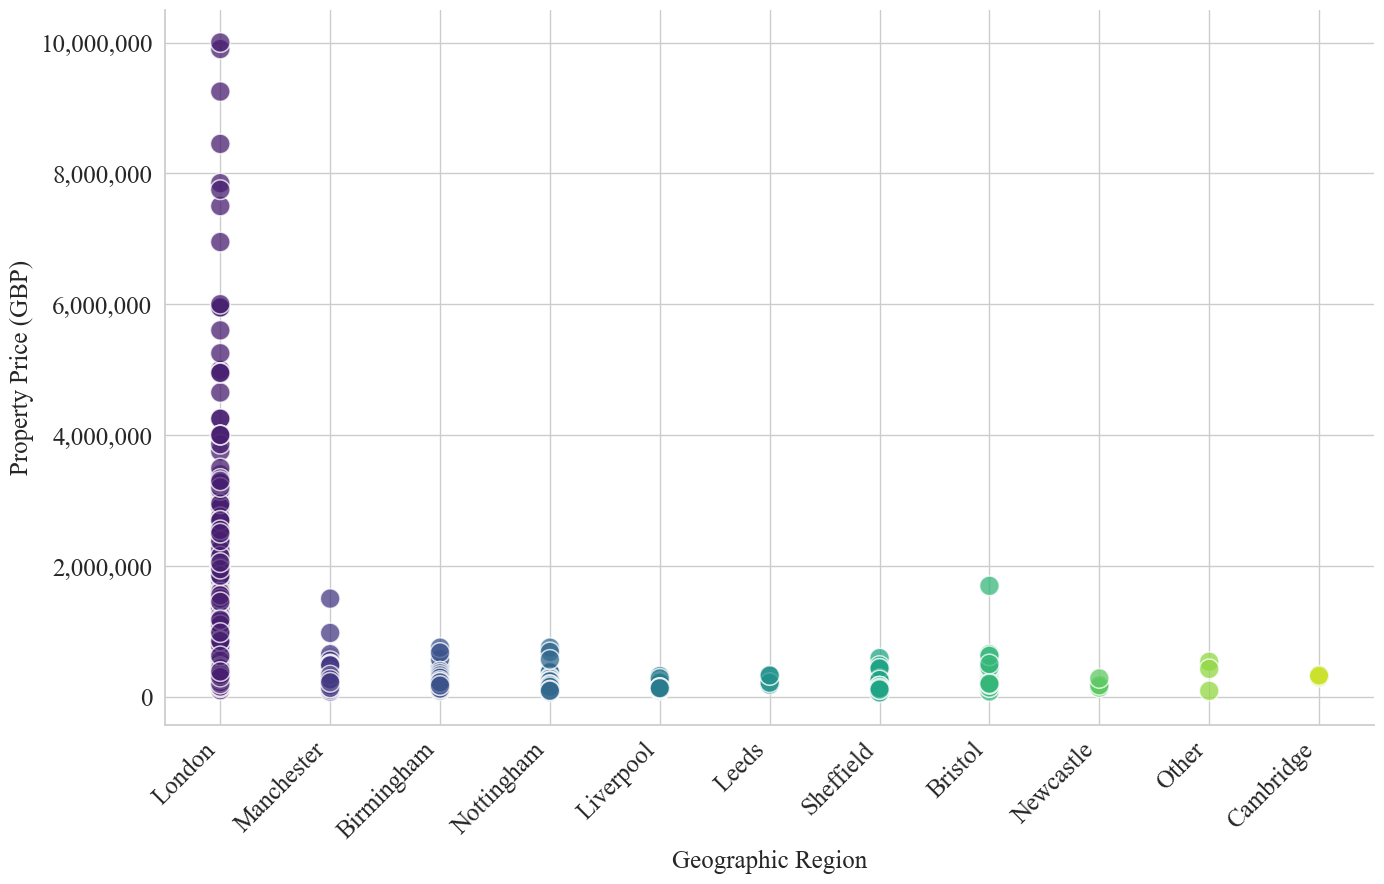
\includegraphics[width=\textwidth]{impl/images/distribution.png}
    \caption{Properties Prices distributed by Region.}
    \label{fig:distribution}
\end{figure}

Together, these transformations \textbf{reduce noise, improve distributional assumptions, and provide the model with richer, more discriminative inputs}; all of which contribute to more accurate and generalisable predictions across diverse property types and locations.


\section{Model Training and Evaluation}

With the cleaned and engineered feature set in place, the valuation model for properties prices using XGBoost was implemented.

The model was trained to predict the logarithmic value of the price of the property, using the processed features as input. Data were split using standard 80\% training and 20\% testing split returned from \verb|sklearn.model_selection.train_test_split| \parencite{ScikitLearn2025}.

With \verb|random_state=42| \parencite{Ahmed2022} used to keep the split reproducible between repeated runs. This was helpful during development because it meant that changes in performance or behaviour could be traced back to changes in the pipeline itself rather than differences in the train-test split. The final model was implemented as an \texttt{XGBRegressor} \parencite{DistributedDeepMachineLearningCommunity2026} with a \texttt{random\_state=42}, making the model reproducible.

\begin{minted}[
    bgcolor=gray!8,
    linenos=true,
    fontsize=\small,
    frame=single,
    rulecolor=gray!40
]{python}
from xgboost import XGBRegressor

model = XGBRegressor(
    n_estimators=500,
    learning_rate=0.05,
    max_depth=8,
    subsample=0.8,
    colsample_bytree=0.8,
    random_state=42,
    eval_metric='rmse'
)
\end{minted}

These parameters were not determined through exhaustive searches of all possible combinations. Although a more comprehensive tuning process could have been conducted, it would have significantly increased the time required without necessarily altering the broader contribution of the project, which relies as much on explainability and integration as on raw predictive optimisation. 

Moreover, such extensive tuning was unnecessary because the default parameter configuration already yielded a high-level \textbf{estimating model with an accuracy of 0.9557}.

Upon completion of the final model training, both the regression trained model and the feature column list were preserved as \verb|pickle| files. The preservation of both files is essential for the explanatory SHAP model and for the web application prediction architecture.

This approach facilitated a clear delimitation between the notebook-based training phase and the web application layer. Consequently, the backend loads the saved artefacts, eliminating the need to re-execute the training code or reconstruct the training environment during runtime.

Although the notebook also includes held-out testing and metric calculation, the results are addressed in the relevant Chapter \ref{ch:Evaluation} \nameref{ch:Evaluation}.

\section{SHAP Explanation Layer}
\label{se:SHAPExplanationLayer}

The explanation pipeline was implemented across two components: the module encapsulating the core 
inference and attribution logic, and the dedicated route exposing this functionality to the frontend. 
The explainer loads the persistent XGBoost model along with the stored feature column list, reconstructs the input feature vector from a dictionary of property attributes, and applies \verb|shap.TreeExplainer|\parencite{shap2026} to generate local feature-attribution values for each prediction.

A critical requirement during this phase was to ensure that the inputs supplied at deployment were subjected to identical preprocessing to that applied during training. This included reconstructing one-hot encoded columns for postcode area and property type, inserting any absent columns as zeros, and reordering the feature vector to match the training schema; which is defined inside the \verb|predict_and_explain(input_features: dict)| function. Failure to enforce this consistency would have compromised the reliability of the SHAP attributions and would risk producing erroneous output. 

Consequently, a substantial portion of the explanation logic is dedicated to input validation and structural reconstruction, rather than the attribution computation itself.

A further consideration concerns the presentation of SHAP outputs to end users. Raw feature-attribution values, whilst informative for technical inspection, are not readily interpretable by a general audience, and thus, by the end users of this project. To address this, the system was designed to return both the underlying SHAP contribution values and a concise natural-language summary of the prediction rationale. This translation layer between the technical attribution output and the user-facing interface was a deliberate design decision, intended to \textbf{improve the accessibility and interpretability of the system without sacrificing the underlying analytical depth}.


\section{Backend Implementation}

Once the valuation and explanation components were functioning reliably, a FastAPI backend was implemented through Uvicorn and it acted as the primary connection point between the machine learning pipeline and the frontend web application. Its role was to serve listing data from the CSV dataset, load the persisted model artefacts, accept property inputs from the web application, and return predictions and explanations.

The main backend file is \verb|app.py|, which defines the FastAPI application, request schema, utility functions, and API routes. In addition, a \verb|PropertyInput| class was used to specify the fields expected for prediction and explanation requests, based on the features that were used during the training of the XGBoost regression model. In practice, using a defined request model improved consistency and made testing easier because the API always expects a stable structure.

The backend architecture incorporates distinct routes, namely \verb|/predict| and \verb|/explain|. The \verb|/predict| route exclusively returns the predicted value for a property given the features that make up it, whereas the \verb|/explain| route provides a comprehensive output, including the predicted value, the base price, the SHAP breakdown and concise human-readable explanatory text.

Additional routes were implemented to facilitate direct access to the properties records in the dataset, specifically \verb|/api/properties|, \verb|/api/property/{uprn}| requiring the Unique Property Reference Number (UPRN) and \verb|/api/risk-data-csv|. These routes were instrumental in supporting the frontend browsing, detail view, and risk analysis functionalities, allowing the system to function beyond a mere prediction endpoint.

Together, these components established a structured and extensible backend architecture capable of serving both predictive and explanatory outputs alongside raw listing data, forming the foundational communication layer between the machine learning pipeline and the deployed PropertyIQ web application.


\section{Frontend Implementation}

The final implementation phase concerned the development of the frontend, which translated the backend functionality into an accessible web application. The interface was constructed using React and Vite, organised as a single-page routed application with dedicated views for the dashboard, property listings, analysis, property details, and a system explanation page. This structure reflects the overarching objective of this project as a decision-support tool rather than a purely predictive demonstration.

Navigation between views was managed through the React Router, whilst Axios\parencite{Axios2025} facilitated communication with the backend API. Tailwind CSS was used for rapid interface development, and Recharts was used where visual representations offered greater clarity than textual or tabular alternatives. The dedicated explanation page was of particular significance, as it surfaces the underlying system architecture to the user rather than concealing the decision-support process behind the interface, a choice that directly reinforces the transparency objectives of this project.

Certain elements of the initial specification were refined during development, most notably the range of features used for modelling and the complexity of the generated explanatory text. These adjustments were pragmatic in nature and did not compromise the fundamental scope of the project. The resulting system successfully achieved its central objective by integrating property valuation with explainability in a functional, demonstrable artefact, fulfilling the requirements of providing predictive functionality through a backend API and presenting results through a browser-based interface.

\chapter{Evaluation \& Testing}
\label{ch:Evaluation}


\section{Testing Methodology}

The testing programme was structured around two guiding principles. First, the evaluation of the supervised XGBoost regression model was conducted on data withheld from the fitting process, ensuring that reported performance figures reflect generalisation capability rather than  memorisation of training the training samples. Second, the explanation layer requires an independent testing discipline, since the correctness of its output cannot be inferred from the predictive accuracy of the underlying SHAP model alone. 

Four categories of tests were conducted: quantitative performance evaluation of the predictive model against a held-out test partition; behavioural testing of the explanation layer through additivity, consistency, and directional credibility cheques; integration testing of the end-to-end prediction pipeline via the FastAPI endpoints; and usability evaluation conducted with 
prospective end-users.

Beyond quantitative and behavioural testing, the fully integrated application was evaluated through structured user testing sessions, reflecting the project objective of assessing how end-users perceive and interact with the final deliverable. Participants were presented with the complete system that encompasses price prediction, SHAP-based feature attribution, and the frontend interface  and asked to complete a series of predefined scenarios representative of realistic usage. Feedback was collected following each scenario to capture both task performance and subjective user perception, including the interpretability of the model's explanations and the overall usability of the interface.


\section{Predictive Performance}

The cleaned and encoded dataset was partitioned into a 80\% training set and a 20\% evaluation set using the \verb|scikit-learn| \verb|train_test_split()| function.

The model achieved a Coefficient of Determination ($R^2$) of 0.9557 in the held-out partition, indicating that the fitted estimator accounts for approximately 95.57\% of the variance in the log-transformed price variable across unseen listings.

To complement the statistic $R^2$, the Mean Absolute Error (MAE) was calculated in the logarithmic transformed target space and subsequently inverted to the pound-sterling scale, producing a value of \pounds56,451. Given that the training data include high-value residential properties, this margin represents a reasonable absolute error relative to the typical price range of the considered listings.

\subsection{Limitations and Transparency}

Although the model achieves a strong $R^2$ of $0.9557$ and an MAE of \pounds56,451, it is important to recognise that the predictions carry inherent uncertainty and should not be treated as definitive valuations. The training dataset comprises 977 properties scraped from Zoopla, which introduces selection bias; the model reflects the distribution of listings available at the time of scraping rather than the full breadth of the UK property market. 

Features such as neighbourhood desirability, property condition, and recent local market shifts are not captured in the dataset, meaning that the model can systematically predict certain properties with inaccuracy. To mitigate the risk of misleading users, PropertyIQ presents ML predictions alongside the asking price and SHAP-derived feature explanations, making the reasoning behind each estimate transparent and auditable. Users are implicitly \textbf{discouraged from treating the predicted value as a ground truth and instead are guided to use it as one data point within a broader investment decision-making process}.


\section{SHAP Explanation Layer Review}

The explanation layer was evaluated against three properties whose correctness the broader system depends upon and which cannot be derived from predictive performance alone. The additivity was verified by confirming that the aggregated SHAP values were aligned, with numerical precision, with the difference between the model output and the expected base value; a result that is theoretically guaranteed by \verb|TreeExplainer|, which computes exact Shapley values rather than sampling-based approximations. 

Consistency was established by confirming that repeated calls to \verb|predict_and_explain| with identical inputs produced exactly identical decompositions in all iterations. Although directional credibility was assessed through controlled feature perturbations: increasing gross internal floor area produced positive SHAP contributions; reducing years remaining on a leasehold below standard 
thresholds produced negative contributions; and substituting the postcode sector between central London and regional identifiers produced the expected shift in locational attribution. 

In each case, the observed behaviour was consistent with the hedonic pricing relationships discussed in Section \ref{ch:Background} \nameref{ch:Background}.


\section{User Testing}

To complement the quantitative and behavioural evaluation reported in the following subsections, a \textbf{user testing exercise was conducted to gather qualitative feedback on how the project pipeline presents itself to potential users} of the PropertyIQ web application, in Figure \ref{fig:webapp}.

\begin{figure}[h]
    \centering
    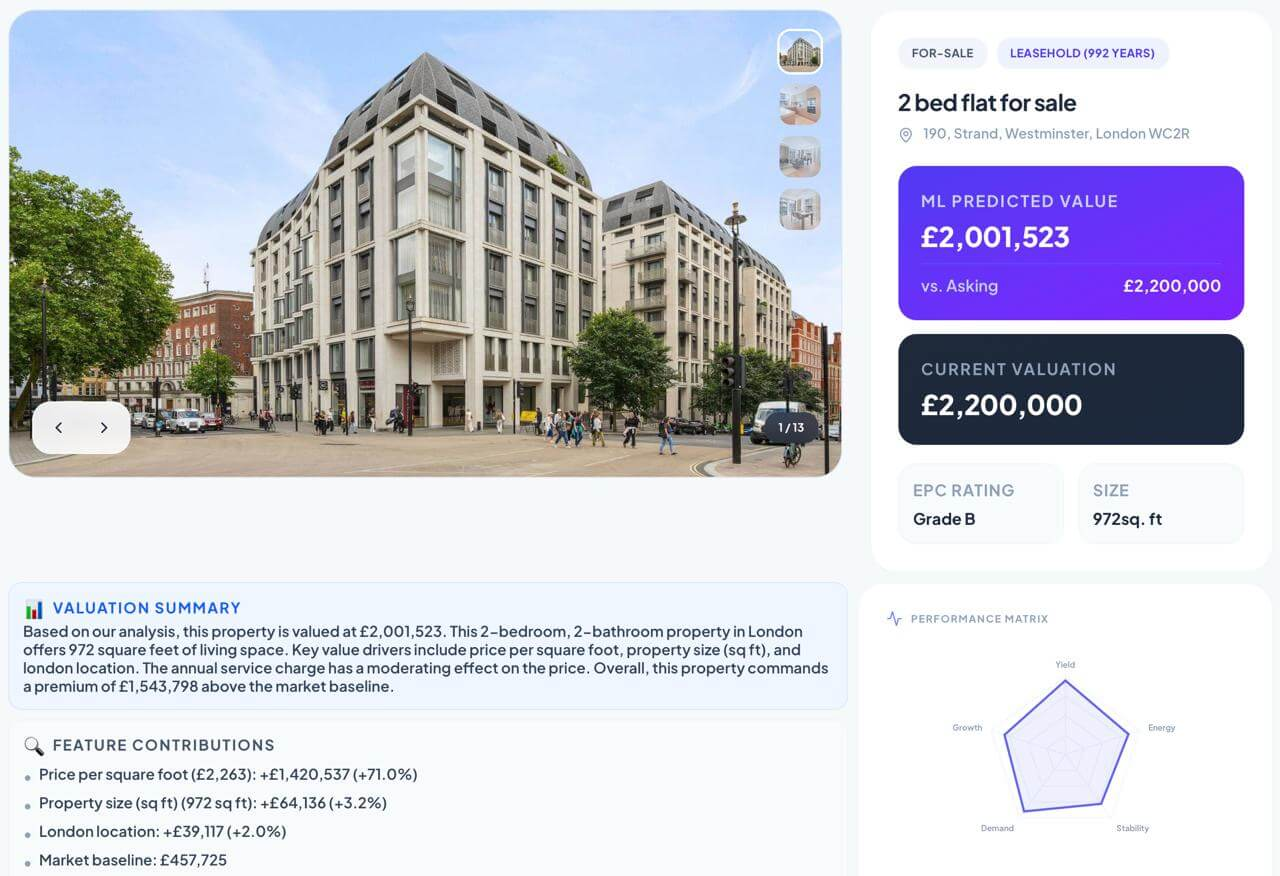
\includegraphics[width=\textwidth]{eval/images/webapp.jpeg}
    \caption{PropertyIQ webapp with predicted value and explanation.}
    \label{fig:webapp}
\end{figure}


\subsection{Small-scale individual property investor}
\label{su:SmallScaleInvestor}

The first participant was a small-scale individual investor who had a modest residential portfolio with no prior exposure to explainability-based tools of the kind developed in this project. Their response was informed by the contrast between the platform and their current practice, which requires them to perform due diligence on each property manually to assess whether the asking price represents fair value. 

The prospect of obtaining a decomposed valuation at the click of a button, in place of a process they estimated at approximately two hours of work per property, was described as a substantial improvement on their current workflow and constitutes one of the clearest articulations of the efficiency gain the pipeline is capable of delivering for individual investors.

The participant also responded with notable enthusiasm to the risk early warning component, which is identified in Section \ref{se:FutureWork} \nameref{se:FutureWork}. They explained that as holders of illiquid residential assets, they have no continuous means of evaluating the condition or current value of their holdings and must engage a professional surveyor at a significant cost whenever such an assessment becomes material. 

In their view, a platform capable of surfacing risk indicators against properties already owned was a natural and commercially valuable extension of the core valuation tool. Their feedback also included a concrete feature suggestion, namely a side-by-side comparison mode in which two properties could be evaluated against each other, and a recommendation surfaced as to which represented the strongest proposition, a suggestion that aligns with the tradition of comparative assessment described in Section \ref{se:GeneralBenfits} \nameref{se:GeneralBenfits}.

The only reservation offered concerned the depth of the explanation layer itself, with the participant indicating that a more detailed accompanying text would further improve the interpretability of individual feature contributions. However, in general, the session was markedly positive, and the participant expressed confidence in the near-term prospects of such a platform.


\subsection{Prospective first-time buyer}

The second participant was actively considering their first residential purchase and had no previous exposure to such tools. Once the conceptual basis of the platform was explained, a predictive valuation was paired with a feature-level account of how that valuation was generated. 

Their response was enthusiastic, and the reasoning they offered for that enthusiasm merits recording in some detail, as it speaks directly to user-trust motivations. They described the difficulty of evaluating individual properties without a reliable reference point and reported a repeating experience in which selling agents, when pressed on the basis of an asking price, deflected the question on the grounds that they were only representing the seller's stated figure rather than justifying it. 

The prospect of a tool capable of decomposing a valuation into its constituent drivers was, in their words, materially useful to someone preparing to make their first purchase.
The feedback, following the interactive session, was consistent with the initial reaction. The participant engaged positively with the SHAP-generated explanation layer, describing it as the element that distinguished the platform from the conventional listing-based tools they had previously encountered. 

The simplified interface and general visual presentation of the application were each praised, and the participant made repeated use of the prediction functionality against the set of integrated properties to develop a better understanding of how the contributions of features shifted across comparable listings. Their principal reservation, offered as a constructive feature, concerned the depth of the natural-language explanation itself: while the concept and its execution were well received, the participant expressed a preference for longer and more granular explanatory text, particularly for features they did not immediately recognise.


\section{Evaluation}

The testing demonstrated that PropertyIQ met most of the objectives set in Appendix \ref{ch:Specifications} \nameref{ch:Specifications}. The predictive ML model performs at a level broadly consistent with the benchmarks reported for tree-based ensemble methods in the property valuation literature \parencite{Ho2020} \parencite{Rico-Juan2021}.
The explanation layer produces attributions that are mathematically accurate, reproducible on repeated calls, and directionally consistent with the hedonic pricing relationships. In general, these outcomes support the view that the system occupies a credible middle ground between predictive accuracy and interpretability, which the literature review identified as the central trade-off confronting ML evaluation tools.

Integration testing against the FastAPI endpoints confirmed that the valuation and explanation pipelines behaved consistently when invoked through the same interface used by the frontend. This distinction is significant because the preprocessing logic that reconstructs the feature vector at inference time introduces a class of errors that would remain hidden during offline evaluation. 

No discrepancies were observed between notebook and endpoint-based predictions on matched inputs, suggesting that the separation between training artefacts and deployed application was implemented with sufficient precision to preserve the integrity of the attribution results.

Although limited in scale, the usability sessions served as a corrective to the assumption that technical correctness alone is sufficient for a decision-support system. Participants were able to interpret the natural-language summaries accompanying each assessment but reported greater difficulty with the raw SHAP contribution values, which reinforces the design decision made in Section \ref{se:SHAPExplanationLayer} \nameref{se:SHAPExplanationLayer} to expose both representations rather than relying on the attribution figures in isolation. 

The evaluation therefore supports the conclusion that PropertyIQ succeeds as an integrated artefact rather than merely as a pair of functioning models, while also identifying the presentation of explanations as the area in which further refinement is most warranted.

\section{Challenges Encountered}

This section outlines challenges that were encountered during the development of the project and in producing the expected results and artefacts.

One of these challenges was that the one-hot encoded postcode and property-type columns are derived from the categorical values observed during training; any mismatch between the fit-time schema and the feature vector assembled at inference would produce either silent errors or attributions that could not be interpreted meaningfully. 

Preserving strict schema parity by persisting the training feature list alongside the model artefact and reconstructing absent columns as zero-valued entries at inference accounted for a disproportionate share of the explanation-layer implementation effort. 

This is consistent with the observation in Section \ref{se:SHAPExplanationLayer} \nameref{se:SHAPExplanationLayer} that a substantial portion of the explanation logic is concerned with input validation rather than the attribution computation itself.

Translating SHAP generated outputs into a form accessible to non-technical users was more difficult than anticipated. Although raw attribution values are mathematically precise, they do not intuitively map onto the qualitative reasoning that a prospective buyer or small-scale investor is likely to apply when assessing a listing. 
Producing concise natural-language summaries that preserve the directional and relative significance of the underlying contributions without overstating the certainty of any individual attribution requires iterative refinement and remains, as acknowledged in Section \ref{se:FutureWork} \nameref{se:FutureWork}, comparatively modest in the current implementation.

The final and more pragmatic difficulty concerns the scope of hyperparameter tuning applied to the XGBoost regressor. An exhaustive search of the parameter space might have yielded marginal gains in predictive accuracy, but the associated computational and time costs were not considered to be proportional to the broader emphasis of this project on explainability and integration. 

The adopted configuration, although not formally optimised, produced a model that met the accuracy requirement set out in Appendix \ref{ch:Specifications} \nameref{ch:Specifications}, and the decision to prioritise the explanation pipeline over further tuning is, in retrospect, consistent with the stated objectives.
\chapter{Conclusion \& Future Work}
\label{ch:Conclusion}

The following sections present the conclusions drawn from PropertyIQ development and evaluation, alongside directions for future research. This section reflects on the extent to which the project objectives were met, and it identifies areas in which the system could be meaningfully extended.


\section{Conclusion}
\label{se:Conclusion}

This project investigated the extent to which a property valuation system could be enhanced by integrating explanatory mechanisms with its predictions. The resulting prototype, PropertyIQ, combines a trained XGBoost valuation model, SHAP-based attribution, a Python backend, and a React frontend into a unified system capable of presenting property listings, generating valuations, and communicating the rationale underlying those valuations. In doing so, \textbf{this project advances beyond a conventional ``black-box'' approach towards a more transparent decision-support tool}.

A principal finding of this project is that explainability yields practical value only when it is meaningfully integrated into a larger system. A model explanation is not inherently useful by virtue of its existence; it must be presented in a form that users can interpret in relation to the specific properties under consideration. Consequently, the frontend interface and clear interpretation view were of comparable importance to the machine learning model itself. The most significant outcome was therefore not the integration of SHAP with a valuation model in isolation, but the \textbf{capacity to embed that explanation within a coherent, user-facing workflow}.

The project also demonstrated that effective property intelligence systems cannot be constructed using a singular reasoning approach. Within PropertyIQ, certain outputs were determined statistically via the XGBoost regression model, whilst others were addressed through the web application user interface. This combination made the system more interpretable and functional than a model-only implementation. In general, this project illustrates both the feasibility of an explainable property valuation and the considerable potential for further development within this domain.


\section{Future Work}
\label{se:FutureWork}

An avenue for future development lies in \textbf{broadening the scale of the dataset and the range of features available to the model}. Although the project relied on genuine property listings, the dataset used for the modelling was limited in size and the variables contained were largely limited to those directly available from the scraped source. A logical extension would be to incorporate additional location and neighbourhood-level attributes, including accessibility to transport, local market demand indicators, school performance metrics, and crime statistics, provided that these can be sourced and matched to individual properties with reasonable reliability. Expanding the feature space in this manner would likely improve both the accuracy of the valuations and the contextual richness of the accompanying explanations.

A further extension would involve the introduction of a dedicated user account system that would allow individuals to register, authenticate, and manage a portfolio of personal property within the platform. This would transition PropertyIQ from a tool supporting one-off valuations to a longitudinal decision-support system for prospective buyers and small-scale investors. This would substantially increase the practical utility of the platform by supporting both the evaluation of individual listings and the ongoing management of investment risk across a broader portfolio.

Furthermore, a natural extension of PropertyIQ's existing risk intelligence capabilities would be the introduction of a proactive early warning system tailored to individual user portfolios. Rather than requiring users to manually inspect each asset, this feature would continuously monitor key indicators, such as shifts in local market valuations, deteriorating EPC ratings relative to upcoming regulatory thresholds, and lease term erosion; and automatically surface properties exhibiting signs of value decline. Using the existing XGBoost model alongside time-series trend analysis, the system could generate personalised alerts ranked by severity, enabling investors to act before depreciation becomes significant.

Lastly, a valuable addition would be a dedicated property comparison interface, which would allow users to evaluate two or more listings against each other using a structured, side-by-side layout. This feature was suggested and considered during the user testing phase as described in Section \ref{su:SmallScaleInvestor} \nameref{su:SmallScaleInvestor}. Beyond raw listing attributes such as price, size, and EPC rating, the view would surface the model's SHAP-derived feature contributions for each property, making it immediately clear which asset offers stronger value drivers and which carries greater risk exposure. This would directly address the information asymmetry problem central to PropertyIQ's mission, giving investors an explainable, data-grounded basis for prioritising one acquisition over another without having to cross-reference multiple pages manually.
\include{usingLatex/usingLatex} % NOTE: Before compiling your final document, please don't forget to "comment this section". That is, adding a %  before the \include to omit it, as this section only contains the instructions and a sample on how to use this template

\footnotesize % NOTE: reduced the size of the text for the bibliography
%N OTE: set the style for the bibliography and display the references used within the document

\printbibliography
\normalsize

% If you are not using an appendix, comment the following two lines
\appendix
\chapter{Project Specification}
\label{ch:Specifications}

The following requirements have been defined to guide the development and implementation of the ML model for the PropertyIQ web application.

\section{Functional Requirements}

\begin{enumerate}
    
    \item Must take in a dataset of real residential property listings and convert it into a format that a supervised ML pipeline can work with, given the inconsistent and ``string'' nature of fields typically found in scraped listings.
    
    \item Must clean the input data so that malformed entries, inconsistent encodings, or missing values do not corrupt the training process or distort the model's learning behaviour.
    
    \item Must split the prepared data into separate training and evaluation subsets, in line with standard practice for supervised regression tasks, so that the reported performance reflects how the model generalises rather than how well it memorises the data.
    
    \item Must train a regression model that learns to map a set of property features to a continuous estimate of monetary value; Random Forest and XGBoost are perfect candidates as highlighted in Section \ref{se:MLBackground} \nameref{se:MLBackground}.

    \item Must return a valuation for any valid feature vector given at inference time, with the output expressed in the same currency units as the training data.

    \item Should encode categorical attributes, such as those describing location and property type, in a way that preserves their meaning whilst remaining usable by the chosen learning algorithm.

    \item Should report its predictive performance on held-out data using regression metrics that convey both relative and absolute error, so that the quality of the model can be judged on more than a single figure.

    \item Could go beyond the attributes directly available in the source data by deriving additional features from unstructured or semi-structured fields, where these can be shown to add value.

\end{enumerate}


\section{Non-Functional Requirements}

\begin{enumerate}

    \item Must reach a level of predictive performance in line with what has been reported for current machine-learning approaches to property valuation, so that its output can reasonably be used to inform user decisions rather than serve only as a rough indication.

    \item Must lend itself to post-hoc explanation through feature-attribution techniques, in keeping with the transparency arguments set out in the literature review, so that the second stage of PropertyIQ can break each prediction down into the contributions of its individual inputs.

    \item Must return equivalent results across repeated runs on the same inputs, both to support academic verification and to meet the reliability expectations of an application intended for real use.

    \item Should be usable by the wider PropertyIQ web application through a clearly defined interface, independently of the notebook in which it is developed, so that the research artefact can move into a deployable form without structural rework.

    \item The pipeline should be broken into distinct stages with clear boundaries between them, which allows any one part to be adjusted, swapped out, or expanded without pulling the rest of the pipeline apart.

    \item Could respond in a controlled and predictable way when faced with incomplete or unexpected input, rather than producing silent failures or valuations that make no sense given the circumstances.
    
\end{enumerate}


\chapter{Project Log}
\label{ProjectLog}

The following is a weekly summary of the work carried out during the development of the ML model and PropertyIQ web application. It covers tasks that were completed, tutorials that were worked through, articles that were read, and reviews of discussions / meetings held with the project supervisor and other third parties. 

\section*{Week One: Thursday 12/02/2026}
Initial meeting with this project supervisor, scoped the problem space around property analytics and machine learning. 
\begin{itemize}
  \item Discussed several candidate project directions, with an emerging focus on transparency in property valuation tools and DSS \parencite{Giudice2019}.
  \item Identified the ``black-box'' problem in current property platforms as a meaningful gap worth addressing.
\end{itemize}

\section*{Week Two: Thursday 19/02/2026}
Focused on shaping the project's academic grounding through early literature review work.
\begin{itemize}
    \item Reviewed foundational appraisal literature, including \textcite{Rosen1974} \textcite{Pagourtzi2003}, to understand the evolution from sales comparison through to hedonic regression.
    \item Identified the tension between interpretability (hedonic regression models) and predictive accuracy (ensemble ML models) as a central theme of this project.
\end{itemize}

\section*{Week Three: Thursday 26/02/2026}
Continued literature review with a shift towards Machine Learning and XAI.
\begin{itemize}
    \item Reviewed \textcite{Ho2020} \textcite{Rico-Juan2021} \textcite{Kim2025} on ensemble methods outperforming regression in property valuation.
    \item \textcite{Ribeiro2016} on LIME and \textcite{Lundberg2017} on SHAP, which reinforced the decision to pair a predictive model with a dedicated explanation layer.
    \item Started drafting Section \ref{ch:Background} \nameref{ch:Background}.
\end{itemize}

\section*{Week Four: Thursday 05/03/2026}
Continued literature review alongside early design and system architecture work.
\begin{itemize}
    \item Began sketching the overall system architecture: separate ML workspace, backend API, and React frontend.
\end{itemize}

\section*{Week Five: Thursday 12/03/2026}
Finalised design and system architecture, refined the toolchain.
\begin{itemize}
    \item Confirmed the \textbf{initial} tech stack: Python (Pandas and NumPy) for data handling, Fast API for the backend, and React with frontend with interactive visualisations.
    \item Drafted Section \ref{ch:Design} \nameref{ch:Design} chapter, including the rationale for modular separation between presentation and data logic.
    \item Defined the functional and non-functional requirements that later formed Appendix \ref{ch:Specifications} \nameref{ch:Specifications}.
\end{itemize}

\section*{Week Six: Thursday 19/03/2026}
Literature review nearly completed and transitioned into the data preprocessing phase.
\begin{itemize}
    \item Sourced the dataset used for the project: a scraped Zoopla export of 1,000 UK residential listings with 43 raw attributes.
    \item Imported the CSV into Pandas and ran an initial inspection, identifying irrelevant columns (URLs, image links) and sparsely populated fields (virtual tours, deposits, letting arrangements).
    \item Began drafting content for the final report in \LaTeX.
\end{itemize}

\section*{Week Seven: Thursday 26/03/2026}
Poster submission week.
\begin{itemize}
    \item Finalised and submitted the academic poster for PropertyIQ.
    \newline \textbf{\textit{Note}}: the poster represented an earlier iteration of the project and referenced Random Forest (0.89), Django, etc. The technical direction was revised afterwards, and the final system differs significantly from what was presented at the poster.
\end{itemize}

\section*{Week Eight: Thursday 02/04/2026}
Implementation began in earnest, starting with a pivot in the technical approach.
\begin{itemize}
    \item Pivoted from Random Forest to XGBoost, selected for its stronger compatibility with SHAP's TreeExplainer and its proven performance on structured tabular data.
    \item Pivoted from Django to FastAPI served via uvicorn, a lighter-weight choice better suited to the scope of serving predictions and explanations.
    \item Completed the data cleaning pipeline: regex-based stripping of currency symbols from price, normalising service charge, extracting numerical property size, and encoding property type.
    \item Dropped records missing critical fields (price, size), reducing the working dataset from 1,000 to 977 records.
\end{itemize}

\section*{Week Nine: Thursday 09/04/2026}
Core ML pipeline built and validated.
\begin{itemize}
    \item Implemented feature engineering: \verb|price_per_sqft|, \verb|log_price| (via \verb|numpy.log1p|), and one-hot encoded postcode area columns.
    \item Trained the final XGBRegressor, achieving an $R^{2}$ of 0.9557 on the held-out 20\% test partition.
    \item Persisted the trained model and feature column list as \verb|.pkl| artefacts to cleanly decouple training from deployment.
    \item Integrated \verb|shap.TreeExplainer| and wrote the \verb|predict_and_explain| function used in the web application, including the input-validation and feature-vector reconstruction logic required to match the training schema.
\end{itemize}

\section*{Week Ten: Thursday 16/04/2026}
Backend, frontend, evaluation and final writeup.
\begin{itemize}
    \item Built the FastAPI backend (\verb|app.py|) with a \verb|PropertyInput| class working as a request schema and routes for \verb|/predict|, \verb|/explain|, \verb|/api/properties|, etc.
    \item Developed the React frontend with React Router, Axios, Tailwind CSS, and Recharts, covering the dashboard, listings, analysis, property detail and system-explanation views.
    \item Ran evaluation and testing: confirmed $R^{2}$ of 0.9557, MAE of \pounds56,451, and validated SHAP additivity, consistency, and directional credibility through controlled perturbation tests.
    \item Completed the Chapter \ref{ch:Implementation} \nameref{ch:Implementation}, \ref{ch:Evaluation} \nameref{ch:Evaluation} and \ref{ch:Conclusion} \nameref{ch:Conclusion}
\end{itemize}

\section*{Week Eleven: Thursday 23/04/2026}
Finished the project.
\begin{itemize}
    \item Formatted and completed \LaTeX report.
    \item Added Appendix \ref{ProjectLog} \nameref{ProjectLog}.
    \item Review and final upload of the project to the GitHub repository \parencite{Kirilov2026}.
\end{itemize}

\chapter{Source Code}
\label{ch:SourceCode}

The source code for this project; including the Jupyter Notebook model, Python files, and the React website, is available at the following link: \url{https://github.com/milenkirilov888/PropertyIQ}.






\end{document} % NOTE: END of document, nothing after this point
%%%%%%%%%%%%%%%%%%%%%%%%%%%%%%%%%%%%%%%%%%%%%%%%